\chapter{Elementmetoden}

\emph{Elementmetoden}, eller \emph{Finite Element Method} (FEM) er en numerisk metode for å løse partielle differensiallikninger (PDE) som beskriver fysiske fenomener som varmeoverføring, elastisitet, væskestrøm osv.

Kort forklart går metoden går ut på å dele opp domenet i små, enkle geometriske \emph{elementer} (som en linje, trekant, firkant osv.).
Innenfor hvert element tilnærmes løsningen med enkle funksjoner.
Til slutt settes elementene sammen for å få en tilnærmet løsning over hele området.

\section{Fremgangsmåte}
\begin{enumerate}
    \item Finn \(u: \Omega \rightarrow \mathbb{R}\) slik at \(\mathcal{L} u = f\) i \(\Omega\) og \(u\big|_{\partial\Omega} = g\) på randen \(\partial\Omega\).

    \item Finn \(u \in V := \mathcal{H}_0^1(\Omega)\) slik at \(\inner*{\mathcal{L} u,\mathcal{L} \phi}_\omega = \inner*{f, \phi}_\omega \; \forall \phi \in V\).

    \item Finn \(u_h \in V_h \subset V := \mathcal{H}_0^1(\Omega)\) slik at \(\inner*{\mathcal{L} u_h,\mathcal{L} \phi_i}_\omega = \inner*{f, \phi_i}_\omega \; \forall 1\leq i \leq n\).

    \item Løs \(A\symbf{u} = \symbf{f}\) with \(A_{ij} := \inner*{\mathcal{L} \phi_i, \mathcal{L} \phi_j}\).
\end{enumerate}

\begin{enumerate}
    \item \textbf{discretization 1:} Del domain \( \Omega \) inn i enkle geometriske elementer \( \Omega_e \) og tilnærme løsningen med en lineærkombinasjon av basisfunctioner:
          \[
              u(x) \approx \sum_{i=1}^N c_i \phi_i(x)
          \]
    \item \textbf{weakformulation:} Multipliser differensiallikningen med en testfunksjon \( v(x) \) og integrer over domainet \( \Omega \):
          \[
              \int_\Omega v(x) \mathcal{L}(u) \, dx = \int_\Omega v(x) f(x) \, dx
          \]

    \item \textbf{Galerkin-prosedyre:} Tilnærme løsningen og testfunksjonen med basisfunctioner:
          \[
              u(x) \approx \sum_{i=1}^N c_i \phi_i(x) \quad \text{og} \quad v(x) \approx \sum_{j=1}^N d_j \phi_j(x)
          \]
    \item \textbf{discretization 2:} Sett inn tilnærmingene i den svake formen og diskretiser:
          \[
              \sum_{j=1}^N d_j \int_\Omega \phi_j(x) \mathcal{L} \left( \sum_{i=1}^N c_i \phi_i(x) \right) \, dx = \sum_{j=1}^N d_j \int_\Omega \phi_j(x) f(x) \, dx
          \]
    \item \textbf{Matriseform:} Skriv den diskretiserte formen som et ligningssett:
          \[
              \symbf{K} \symbf{c} = \symbf{F}
          \]
          Og løs ligningssystemet for å finne koeffisientene \(c_i\):
          \[
              \symbf{c} = \symbf{K}^{-1} \symbf{F}
          \]
\end{enumerate}

\begin{enumerate}
    \item \textbf{Definer problemet:} Finn pde, over hvilket domene og rand.
          \[
              u: \Omega \to \mathbb{R}, \quad \mathcal{L}(u) = f(x) \quad \text{for } x \in \Omega \quad \text{og} \quad u|_{\partial \Omega} = g
          \]
    \item \textbf{Diskretiser domenet:} Del opp \(\Omega\) i enkle geometriske elementer.
    \item \textbf{Lokal approksimering for hvert element:} Innenfor hvert element (ukjente området/løsning) tilnærmer vi løsningen med en lineærkombinasjon av basisfunksjoner.
          \[
              u(x) \approx \sum_{i=1}^N c_i \phi_i(x)
          \]
    \item \textbf{Fra Sterk til Svak formulering:} Formuler pde på weakformulation.
          \[
              \int_\Omega v(x) \mathcal{L}(u(x)) \, dx = \int_\Omega v(x) f(x) \, dx
          \]
          \[
              u \in \mathcal{C}^2 \quad \text{s.t.} \quad \mathcal{L}(u) = f \text{ for } x \in \Omega, \; u|_{\partial \Omega} = g
              \implies
              u \in V \quad \text{s.t.} \quad \inner*{\mathcal{L}(u), \mathcal{L}(\phi)} = \inner*{f, \phi} \; \forall \phi \in V
          \]
    \item \textbf{Formuler elementeneligningene:} Sett sammen elementene til et system av ligninger, ved å bruke weakformulation av pde.
          \[
              \symbf{K} \symbf{u} = \symbf{F}
          \]
    \item \textbf{Randbetingelser:} Sett opp ligningssystemet med randbetingelser.
    \item \textbf{Løs ligningssystemet:} Løs ligningssystemet for å finne koeffisientene \(u_i\).
          \[
              \symbf{u} = \symbf{K}^{-1} \symbf{F}
          \]
\end{enumerate}

\section{Elementrom og basisfunksjoner}
\subsection[Definisjon av elementrom]{Definisjon av elementrommet \(\mathcal{X}_h^p \subset H^1(\Omega)\)}
Finite Element Space \(\mathcal{X}_h^p\) er et rom av stykkvis polynomer av grad \(p\) begrenset på elementet \(\mathcal{K}_i \in \mathcal{T}_h \subset \Omega\).
Hvor \(\mathcal{T}_h\) er en partisjon av domenet \(\Omega\) i elementer \(K_i\).
\begin{example}{Elementer}{elements}
    Eksempler på elementer er trekanter, firkanter, tetraedre osv.
\end{example}
\begin{definition}{Finite Element Space}{lagrange_space}
    \begin{equation}
        \mathcal{X}_h^p = \{v \in \mathcal{C}^0(\Omega) \mid v\big|_K \in \mathrm{P}_p \text{ for alle } K_i \in \mathcal{T}_h\}
    \end{equation}
    \begin{itemize}
        \item $u \in \mathcal{C}^0(\Omega)$ betyr at $u$ er kontinuerlig \(\mathcal{C}^0\) i domenet \(\Omega\).
        \item $v\big|_K \in \mathrm{P}_p$ betyr at $v$ er et polynom av grad \(p\) i elementet \(K\).
        \item \(\mathcal{T}_h\) er en partisjon av domenet \(\Omega\) i elementer \(K\).
    \end{itemize}
\end{definition}
\subsection{Valg av basisfunksjoner}
En sentral del av FEM-metoden er valget av basisfunksjoner for å representere løsningen. Disse funksjonene danner fundamentet for approksimeringen av løsningen i det diskrete rommet.

\subsubsection{Egenskaper til basisfunksjoner}
Basisfunksjoner er funksjoner som brukes til å representere den approksimerte løsningen \(u_h\) i det diskrete rommet \(\mathcal{X}_h^p\).
Gode basisfunksjoner for FEM har følgende egenskaper:
\begin{itemize}
    \item \textbf{Lokal støtte}: \(\phi_i(x) = 0\) utenfor elementene der node \(i\) inngår
    \item \textbf{Interpolasjon}: \(\phi_i(x_j) = \delta_{ij}\) (Kronecker delta)
    \item \textbf{Partisjon av enheten}: \(\sum_{i=1}^n \phi_i(x) = 1\) for alle \(x \in \Omega\)
    \item \textbf{Kontinuitet}: Basisfunksjonene er kontinuerlige på tvers av elementgrensene
    \item \textbf{Representasjon}: Gir en god approksimering \(u_h(x) = \sum_{i=1}^n u_i \phi_i(x)\)
\end{itemize}

Med disse egenskapene kan vi representere enhver funksjon \(v \in X_h^p\) som:
\[
    v(x) = \sum_{i=0}^{M} v_i \phi_i(x) \in \mathbb{P}_p
\]

\subsubsection{Lagrange-basisfunksjoner}
Lagrange-basisfunksjoner er den mest brukte typen polynomielle basisfunksjoner i FEM. De er spesielt praktiske fordi koeffisientene \(u_i\) direkte representerer funksjonsverdiene ved nodene.

\begin{definition}{Lagrange-basisfunksjoner}{lagrange_basis_def}
    Lagrange-basisfunksjoner av grad $p$ er definert ved interpolasjon over nodepunkter $\{x_i\}_{i=0}^{p}$. For hvert nodepunkt $i$, er den tilsvarende Lagrange-basisfunksjonen $\ell_i(x)$ gitt ved:
    \begin{equation}
        \ell_i(x) = \prod_{j=0, j \neq i}^{p} \frac{x - x_j}{x_i - x_j}
    \end{equation}
    med egenskapene:
    \begin{enumerate}
        \item $\ell_i(x_j) = \delta_{ij}$ (Kronecker-delta)
        \item $\ell_i(x)$ er et polynom av grad $p$
        \item $\sum_{i=0}^{p} \ell_i(x) = 1$ for alle $x$ (partisjon av enheten)
    \end{enumerate}
\end{definition}

Lagrange-basisfunksjoner har flere fordeler i FEM:
\begin{itemize}
    \item De gir en direkte tolkning av koeffisientene som funksjonsverdier ved nodene
    \item De forenkler håndteringen av randbetingelser
    \item De har kompakt støtte, noe som gir sparse matriser i implementeringen
\end{itemize}

\paragraph{Lagrange-basisfunksjoner i 1D}
I én dimensjon er Lagrange-basisfunksjonen for node $i$ definert som:
\[
    \phi_i(x) = \prod_{j=0, j \neq i}^{M} \frac{x - x_j}{x_i - x_j}
\]

\begin{example}{Lineære basisfunksjoner i 1D ($p=1$)}{basisfunksjoner_1d}
    For rommet $\mathcal{X}_h^1$ av stykkvis lineære funksjoner er basisfunksjonene gitt ved:
    \[
        \phi_i(x) =
        \begin{cases}
            \frac{x - x_{i-1}}{x_i - x_{i-1}}, & x_{i-1} < x \leq x_i, \\
            \frac{x_{i+1} - x}{x_{i+1} - x_i}, & x_i < x < x_{i+1},    \\
            0,                                 & \text{ellers}.
        \end{cases}
    \]

    \begin{figure}[H]
        \centering
        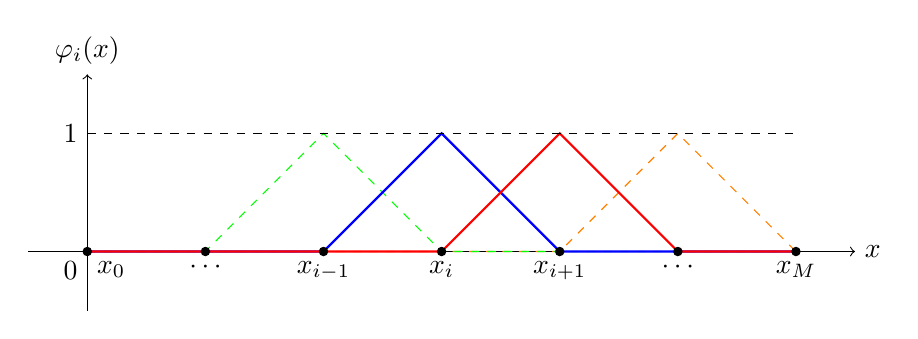
\begin{tikzpicture}[scale=1.5]
            % Axes
            \draw[->] (-1.5, 0) -- (5.5, 0) node[right] {$x$};
            \draw[->] (-1, -0.5) -- (-1, 1.5) node[above] {$\varphi_i(x)$};

            % Basis function
            \draw[orange, dashed] (-1, 0) -- (1, 0) -- (2, 0) -- (3, 0) -- (4, 1) -- (5, 0);
            \draw[green, dashed] (-1, 0) -- (0, 0) -- (1, 1) -- (2, 0) -- (3, 0) -- (4, 0) -- (5, 0);
            \draw[thick, blue] (-1, 0) -- (0,0) -- (1, 0) -- (2, 1) -- (3, 0) -- (4, 0) -- (5, 0);
            \draw[thick, red] (-1, 0) -- (1, 0) -- (2, 0) -- (3, 1) -- (4, 0) -- (5, 0);

            % Nodes
            \filldraw[black] (-1, 0) circle (1pt) node[below right] {$x_0$};
            \filldraw[black] (0, 0) circle (1pt) node[below] {$\cdots$};
            \filldraw[black] (1, 0) circle (1pt) node[below] {$x_{i-1}$};
            \filldraw[black] (2, 0) circle (1pt) node[below] {$x_i$};
            \filldraw[black] (3, 0) circle (1pt) node[below] {$x_{i+1}$};
            \filldraw[black] (4, 0) circle (1pt) node[below] {$\cdots$};
            \filldraw[black] (5, 0) circle (1pt) node[below] {$x_{M}$};


            % Dashed lines
            \draw[dashed] (-1, 1) -- (5, 1);

            % Labels
            \node[below left] at (-1, 0) {$0$};
            \node[left] at (-1, 1) {$1$};
        \end{tikzpicture}
        \caption{Basisfunksjoner $\phi_i(x)$ for $i=0,1,\ldots,M$ i rommet $X_h^1$}
        \label{fig:basis_function}
    \end{figure}

    På et enkelt element $K_i = [x_i, x_{i+1}]$ er bare to basisfunksjoner ulik null:
    \[
        \phi_i(x) = \frac{x_{i+1} - x}{x_{i+1} - x_i}, \quad
        \phi_{i+1}(x) = \frac{x - x_i}{x_{i+1} - x_i}, \quad \text{for } x \in [x_i, x_{i+1}].
    \]

    \begin{figure}[H]
        \centering
        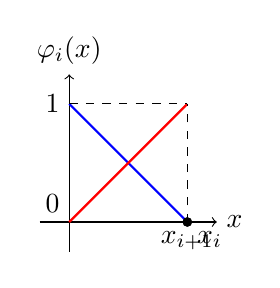
\begin{tikzpicture}[scale=1.5]
            % Axes
            \draw[->] (-0.25, 0) -- (1.25, 0) node[right] {$x$};
            \draw[->] (0, -0.25) -- (0, 1.25) node[above] {$\varphi_i(x)$};

            % Basis function
            \draw[thick, blue] (0, 1) -- (1, 0);
            \draw[thick, red] (0, 0) -- (1, 1);

            % Nodes
            \filldraw[black, right=1cm] (0, 0) circle (1pt) node[below right] {$x_i$};
            \filldraw[black] (1, 0) circle (1pt) node[below] {$x_{i+1}$};

            % Dashed lines
            \draw[dashed] (1, 0) -- (1, 1);
            \draw[dashed] (0, 1) -- (1, 1);

            % Labels
            \node[above left] at (0, 0) {$0$};
            \node[left] at (0, 1) {$1$};
        \end{tikzpicture}
        \caption{Basisfunksjoner $\phi_i(x)$ (blå) og $\phi_{i+1}(x)$ (rød) på elementet $K_i = [x_i, x_{i+1}]$}
        \label{fig:basis_function_element}
    \end{figure}

    \textbf{Nøkkelobservasjoner:}
    \begin{itemize}
        \item \textbf{Lokal støtte:} Hver $\phi_i(x)$ er ulik null kun på de to elementene $K_{i-1}$ og $K_i$
        \item \textbf{Partisjon av enheten:} $\sum_{i=0}^{M} \phi_i(x) = 1$ for alle $x \in [x_0, x_{M}]$
        \item \textbf{Interpolerende:} For en funksjon $v(x)$, gir $v_h(x) = \sum_{i=0}^M v(x_i) \phi_i(x)$ den stykkevis lineære interpolasjonen av $v$ på nodepunktene
    \end{itemize}
\end{example}

\begin{figure}[H]
    \centering
    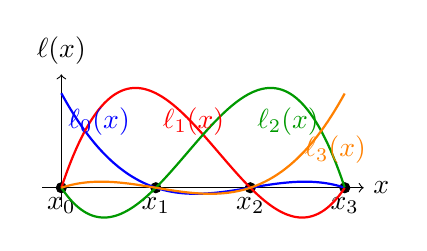
\begin{tikzpicture}[scale=1.2]
        % Axes
        \draw[->] (-0.2,0) -- (3.2,0) node[right] {$x$};
        \draw[->] (0,-0.2) -- (0,1.2) node[above] {$\ell(x)$};

        % Node points
        \filldraw (0,0) circle (1.5pt) node[below] {$x_0$};
        \filldraw (1,0) circle (1.5pt) node[below] {$x_1$};
        \filldraw (2,0) circle (1.5pt) node[below] {$x_2$};
        \filldraw (3,0) circle (1.5pt) node[below] {$x_3$};

        % Cubic Lagrange basis functions
        \draw[thick, blue] plot[domain=0:3,samples=100]
        (\x,{(\x-1)*(\x-2)*(\x-3)/((-1)*(-2)*(-3))});
        \draw[thick, red] plot[domain=0:3,samples=100]
        (\x,{(\x-0)*(\x-2)*(\x-3)/((1-0)*(1-2)*(1-3))});
        \draw[thick, green!60!black] plot[domain=0:3,samples=100]
        (\x,{(\x-0)*(\x-1)*(\x-3)/((2-0)*(2-1)*(2-3))});
        \draw[thick, orange] plot[domain=0:3,samples=100]
        (\x,{(\x-0)*(\x-1)*(\x-2)/((3-0)*(3-1)*(3-2))});

        % Labels
        \node[blue] at (0.4,0.7) {$\ell_0(x)$};
        \node[red] at (1.4,0.7) {$\ell_1(x)$};
        \node[green!60!black] at (2.4,0.7) {$\ell_2(x)$};
        \node[orange] at (2.9,0.4) {$\ell_3(x)$};
    \end{tikzpicture}
    \caption{Kubiske Lagrange-basisfunksjoner ($p=3$) på intervallet $[0,3]$}
    \label{fig:lagrange_basis_cubic}
\end{figure}

Dette kan generaliseres til polynomer av høyere grad ved å bruke flere nodepunkter innenfor hvert element, noe som gir bedre nøyaktighet i løsningen.

\paragraph{Lagrange-basisfunksjoner i 2D}
I to dimensjoner kan Lagrange-basisfunksjoner konstrueres ved bruk av tensorprodukt:

\begin{definition}{Lagrange-basisfunksjoner i 2D}{lagrange_basis_2d}
    \[
        \phi_i(x, y) = \prod_{j=0, j \neq i}^{M} \frac{x - x_j}{x_i - x_j} \cdot \prod_{k=0, k \neq i}^{M} \frac{y - y_k}{y_i - y_k}
    \]
    hvor $(x_i, y_i)$ er nodepunktet i elementet, med egenskapene:
    \begin{itemize}
        \item $\phi_i(x_j, y_j) = \delta_{ij}$ (Kronecker delta)
        \item $\phi_i(x, y)$ er lik null utenfor elementene som inneholder node $i$
        \item $\phi_i(x, y)$ er et polynom av grad $p$ i $x$ og $y$ innenfor hvert element
    \end{itemize}
\end{definition}

For triangulære elementer med lineære basisfunksjoner ($p=1$) brukes ofte barysentriske koordinater, som gir spesielt elegante uttrykk for basisfunksjonene.

\begin{remark}{FEM funksjonsrom}{fem_functionspace}
    Vi må også kreve noe av rommet vi jobber med.
    \[
        V := \{v : v \in \mathcal{C}[0, 1], v^\prime \text{ er stykkvis kont. og bundet på } [0, 1] \text{ hvor } v(0)=v(1)= 0\}
    \]
\end{remark}

\section{fem-betingelser}

\paragraph{Betingelser}

For å bruke fem til å løse et pde-problem, må problemet oppfylle følgende betingelser:

\begin{itemize}
    \item \textbf{Linearitet:} Problemet må være lineært, dvs. ligningene kan uttrykkes som \(\mathcal{L}(u) = f\), hvor \(\mathcal{L}\) er en lineær operator.
    \item \textbf{Kontinuerlig Differensierbar:} Løsningen \( u(x) \) må være kontinuerlig differensierbar i \( \Omega \).
    \item \textbf{Geometrisk Enkelhet:} domainet \( \Omega \) bør kunne deles opp i enkle geometriske elementer (f.eks. trekanter, firkanter i 2D, tetraedre i 3D):
          \[
              \Omega = \bigcup_{e=1}^{E} \Omega_e
          \]
    \item \textbf{Kvantiserbarhet:} Problemet må være kvantiserbart, dvs. løsningen kan tilnærmes godt ved hjelp av en endelig basisfunction:
          \[
              u_h(x) = \sum_{i=1}^{N} c_i \phi_i(x)
          \]
    \item \textbf{Randbetingelser:} Randbetingelsene må være kompatible med valg av funksjonsrom:
          \[
              u|_{\partial \Omega} = g \quad \text{eller} \quad \frac{\partial u}{\partial n}\bigg|_{\partial \Omega} = h
          \]
\end{itemize}

For å anvende fem på en pde, må følgende betingelser være oppfylt:

\subsection{Linearitet} Problemet må kunne uttrykkes i formen \(\mathcal{L}(u) = f\), der \(\mathcal{L}\) er en lineær differensialoperator.

\subsection{Regularitet} Løsningen \( u(x) \) må ha tilstrekkelig regualritet (kontinuitet og differensierbarhet) innenfor \( \Omega \).
\[
    u \in C^2(\Omega) \quad \text{og} \quad u \in C^1(\partial \Omega)
\]

\subsection{Diskretisering av domenet} Domenet \( \Omega \) må kunne dekomponeres i ikke-overlappende elementer:
\[
    \Omega = \bigcup_{e=1}^{E} \Omega_e, \quad \Omega_i \cap \Omega_j = \emptyset \text{ for } i \neq j
\]

\subsection{Approksimering av funksjonsrommet}
Løsningen må kunne representeres tilfredsstillende ved hjelp av basisfunksjoner:
\[
    u(x) \approx u_h(x) = \sum_{i=1}^{N} c_i \phi_i(x)
\]

\subsection{Veldefinerte randbetingelser}
Problemet må ha klart definerte randbetingelser:
\begin{itemize}
    \item Dirichlet-betingelser: \( u = g_D \) på \(\partial \Omega_D \)
    \item Neumann-betingelser: \( \nabla u \cdot \mathbf{n} = g_N \) på \(\partial \Omega_N \)
    \item Robin-betingelser: \( \alpha u + \beta \nabla u \cdot \mathbf{n} = g_R \) på \(\partial \Omega_R \)
\end{itemize}

\section{Sterk formulering}
Gitt $f(x)$, finn $u(x)$ slik at

\begin{align*}
    u^{\prime\prime}(x) & = f(x) \quad \text{for alle } 0 \leq x \leq 1, \\
    u(0)                & = 0,\quad u^{\prime}(1) = 0.
\end{align*}

Introduserer testfunksjonene $v(x)$.
\begin{align*}
    u^{\prime\prime}(x) v(x) & = f(x) v(x)
\end{align*}

Så integrerer vi over intervallet $[0,1]$.
\begin{align*}
    \int_0^1 -u^{\prime\prime}(x) v(x) \, dx & = \int_0^1 f(x) v(x) \, dx
\end{align*}

Alt vi har gjort til nå er å multiplisere med $v(x)$ og integrere over intervallet $[0,1]$, som er generelt lov så lenge $v(x)$ er kontinuerlig og $u(x)$ er to ganger kontinuerlig deriverbar.
Noe den er fra antagelsen om at $u(x)$ er to ganger kontinuerlig deriverbar.

Hvis vi sammenligner integralene på hver side, sier vi egentlig at arealet for $u^{\prime\prime}(x) v(x)$ er lik arealet for $f(x) v(x)$.

\begin{figure}[H]
    \centering
    \begin{minipage}{0.48\textwidth}
        \centering
        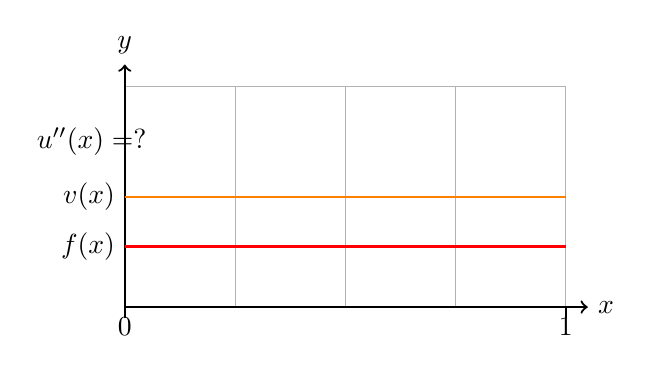
\begin{tikzpicture}[scale=1.4]
            % Grid
            \draw[step=1.0, very thin, black!30] (0,0) grid (4,2);
            \draw[->,thick] (0,0) -- (4.2,0) node[right] {$x$};
            \draw[->,thick] (0,0) -- (0,2.2) node[above] {$y$};
            \draw[thick] (0,-0.1) -- (0,0) node[below] {$0$};
            \draw[thick] (4,-0.1) -- (4,0) node[below] {$1$};

            \draw[orange, thick, domain=0:4, smooth, variable=\x, samples=10] plot (\x, {1});
            \draw[red, thick, domain=0:4, smooth, variable=\x, samples=10] plot (\x, {0.55});

            \node[left] at (0,1) {$v(x)$};
            \node[left] at (0,0.55) {$f(x)$};
            \node[] at (-0.3,1.5) {$u^{\prime\prime}(x) = \displaystyle ?$};
        \end{tikzpicture}
        \caption{Vilkårlig testfunksjon $v(x)$, og kjent $f(x)$}
    \end{minipage}\hfill
    \begin{minipage}{0.48\textwidth}
        \centering
        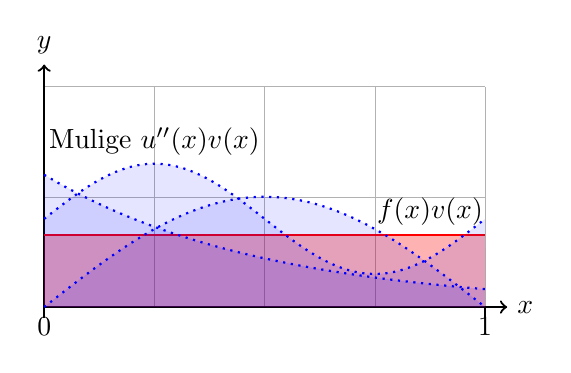
\begin{tikzpicture}[scale=1.4]
            % Grid
            \draw[step=1.0, very thin, black!30] (0,0) grid (4,2);
            \draw[->,thick] (0,0) -- (4.2,0) node[right] {$x$};
            \draw[->,thick] (0,0) -- (0,2.2) node[above] {$y$};
            \draw[thick] (0,-0.1) -- (0,0) node[below] {$0$};
            \draw[thick] (4,-0.1) -- (4,0) node[below] {$1$};

            % Known function f(x)v(x)
            \draw[red, thick, domain=0:4, smooth, variable=\x, samples=100] plot (\x, {0.65});
            \fill[red, opacity=0.3] (0,0) -- plot[domain=0:4, smooth, variable=\x, samples=100] (\x, {0.65}) -- (4,0) -- cycle;

            % Multiple possible u''(x)v(x) functions
            \draw[blue, dotted, thick, domain=0:4, smooth, variable=\x, samples=100] plot (\x, {sin(deg(\x*pi/4))});
            \draw[blue, dotted, thick, domain=0:4, smooth, variable=\x, samples=100] plot (\x, {1.2*exp(-\x/2)});
            \draw[blue, dotted, thick, domain=0:4, smooth, variable=\x, samples=100] plot (\x, {0.8+0.5*sin(deg(\x*pi/2))});

            % Shaded question mark area
            \fill[blue, opacity=0.1] (0,0) -- plot[domain=0:4, smooth, variable=\x, samples=100] (\x, {sin(deg(\x*pi/4))}) -- (4,0) -- cycle;
            \fill[blue, opacity=0.1] (0,0) -- plot[domain=0:4, smooth, variable=\x, samples=100] (\x, {1.2*exp(-\x/2)}) -- (4,0) -- cycle;
            \fill[blue, opacity=0.1] (0,0) -- plot[domain=0:4, smooth, variable=\x, samples=100] (\x, {0.8+0.5*sin(deg(\x*pi/2))}) -- (4,0) -- cycle;

            % Labels
            \node at (1,1.5) {Mulige $u^{\prime\prime}(x) v(x)$};
            \node[above] at (3.5,0.65) {$f(x) v(x)$};
        \end{tikzpicture}
        \caption{Flere mulige løsninger for $u^{\prime\prime}(x)v(x)$, som har samme areal som $f(x)v(x)$}
    \end{minipage}
    \caption{Flere mulige løsninger for $u^{\prime\prime}(x)v(x)$, som har samme areal som $f(x)v(x)$}
    \label{ex:svak_formulering}
\end{figure}

I figur \ref{ex:svak_formulering} er det flere mulige løsninger for $u^{\prime\prime}(x)v(x)$, som har samme areal som $f(x)v(x)$.

I dette tilfellet er testfunksjonen vår $v(x) = 1$ forteller ikke dette oss noe mer om hvordan $u^{\prime\prime}(x)$ ser ut.
Altså det gir oss ikke noe mer informasjon om $u^{\prime\prime}(x)$.

Målet vårt nå er å finne/lage en testfunksjon $v(x)$ som faktisk vil kunne gi oss mer informasjon om $u^{\prime\prime}(x)$.

La oss se på testfunksjonen
\[
    v(x) =
    \begin{cases}
        0 & \text{for } x < a,           \\
        1 & \text{for } a \leq x \leq b, \\
        0 & \text{for } b < x.
    \end{cases}
\]
Denne testfunksjonen er lik $1$ bare i intervallet $[a,b]$ og $0$ ellers, som vist i figuren under.


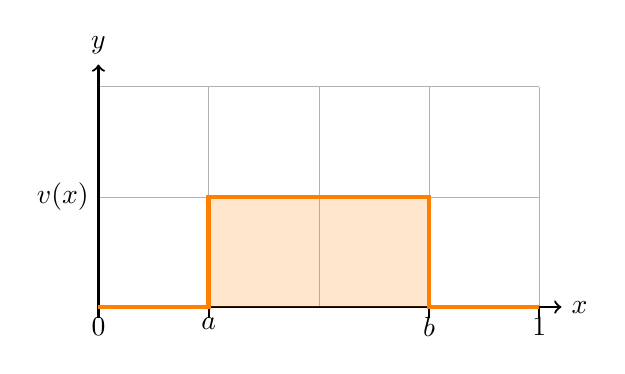
\begin{tikzpicture}[scale=1.4]
    % Grid and axes
    \draw[step=1.0, very thin, black!30] (0,0) grid (4,2);
    \draw[->,thick] (0,0) -- (4.2,0) node[right] {$x$};
    \draw[->,thick] (0,0) -- (0,2.2) node[above] {$y$};
    \draw[thick] (0,-0.1) -- (0,0) node[below] {$0$};
    \draw[thick] (4,-0.1) -- (4,0) node[below] {$1$};

    % Points a and b
    \draw[thick] (1,-0.1) -- (1,0) node[below] {$a$};
    \draw[thick] (3,-0.1) -- (3,0) node[below] {$b$};

    % Test function v(x)
    \draw[orange, ultra thick] (0,0) -- (1,0) -- (1,1) -- (3,1) -- (3,0) -- (4,0);
    \node[left] at (0,1) {$v(x)$};

    % Fill the interval [a,b]
    \fill[orange, opacity=0.2] (1,0) -- (1,1) -- (3,1) -- (3,0) -- cycle;
\end{tikzpicture}

Vi vet at $u^{\prime\prime}(x)$ = f(x) fra den sterke formuleringen. Med vår valgte testfunksjon $v(x)$ får vi:

\begin{align*}
    \int_0^1 u^{\prime\prime}(x) \cdot v(x) \, dx & = \int_0^1 f(x) \cdot v(x) \, dx \\
    \int_0^1 u^{\prime\prime}(x) \cdot v(x) \, dx & = \int_a^b f(x) \cdot 1 \, dx    \\
    \int_0^1 u^{\prime\prime}(x) \cdot v(x) \, dx & = \int_a^b f(x) \, dx
\end{align*}

Merk at integralet på høyre side er begrenset til intervallet $[a,b]$ siden $v(x)=0$ utenfor dette intervallet. På samme måte, på venstre side, bidrar $u^{\prime\prime}(x)$ kun til integralet når $x \in [a,b]$.

En nyttig egenskap ved denne tilnærmingen er at hvis vi lar intervallet $[a,b]$ bli veldig lite, slik at $b \rightarrow a$, kan vi intuitivt tenke at:

\begin{align*}
    \int_a^b u^{\prime\prime}(x) \, dx \approx u^{\prime\prime}(a) \cdot (b-a)
\end{align*}

Tilsvarende for høyresiden:

\begin{align*}
    \int_a^b f(x) \, dx \approx f(a) \cdot (b-a)
\end{align*}

Dette gir oss $u^{\prime\prime}(a) \approx f(a)$ når $b \rightarrow a$, som stemmer med vår opprinnelige differensialligning.

\begin{figure}[H]
    \centering
    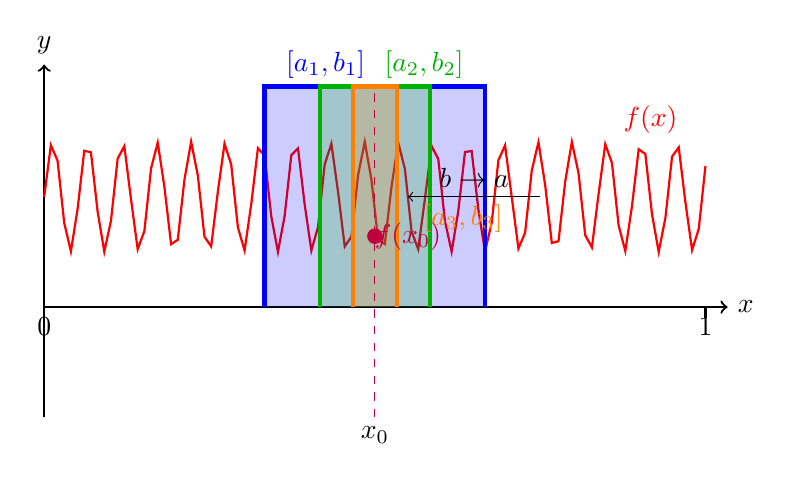
\begin{tikzpicture}[scale=1.4]
        % Axes
        \draw[->,thick] (0,0) -- (6.2,0) node[right] {$x$};
        \draw[->,thick] (0,-1) -- (0,2.2) node[above] {$y$};
        \draw[thick] (0,-0.1) -- (0,0) node[below] {$0$};
        \draw[thick] (6,-0.1) -- (6,0) node[below] {$1$};

        % Functions
        \draw[red, thick, domain=0:6, samples=100] plot (\x, {0.5*sin(deg(\x*20))+1});
        \node[red] at (5.5,1.7) {$f(x)$};

        % Shrinking intervals
        \draw[blue, ultra thick] (2,0) -- (2,2) -- (4,2) -- (4,0);
        \fill[blue, opacity=0.2] (2,0) -- (2,2) -- (4,2) -- (4,0) -- cycle;
        \node[blue, left] at (3,2.2) {$[a_1,b_1]$};

        \draw[green!70!black, ultra thick] (2.5,0) -- (2.5,2) -- (3.5,2) -- (3.5,0);
        \fill[green!70!black, opacity=0.2] (2.5,0) -- (2.5,2) -- (3.5,2) -- (3.5,0) -- cycle;
        \node[green!70!black, right] at (3,2.2) {$[a_2,b_2]$};

        \draw[orange, ultra thick] (2.8,0) -- (2.8,2) -- (3.2,2) -- (3.2,0);
        \fill[orange, opacity=0.2] (2.8,0) -- (2.8,2) -- (3.2,2) -- (3.2,0) -- cycle;
        \node[orange] at (3.8,0.8) {$[a_3,b_3]$};

        % Point identification at limit
        \draw[purple, dashed] (3,-1) -- (3,2);
        \fill[purple] (3,{0.5*sin(deg(3*50))+1}) circle (2pt);
        \node[purple] at (3.3,{0.5*sin(deg(3*50))+1}) {$f(x_0)$};
        \node[below] at (3,-1) {$x_0$};

        \draw[->] (4.5,1) -- (3.3,1) node[midway, above] {$b \rightarrow a$};
    \end{tikzpicture}
    \caption{Når vi gjør intervallet $[a,b]$ stadig mindre, får vi til slutt punktverdien $u^{\prime\prime}(x_0) = f(x_0)$}
    \label{fig:shrinking_interval}
\end{figure}

Men den virkelige styrken med svak formulering kommer når vi bruker delvis integrasjon for å redusere derivasjonsordenene.

\subsection{Delvis integrasjon og svakere krav til regularitet}

La oss nå anvende delvis integrasjon på den svake formuleringen.
Vi har generelt at:

\begin{align*}
    \int_0^1 u^{\prime\prime}(x) v(x) \, dx & = \left. u^{\prime}(x) v(x) \right|_{0}^{1} - \int_0^1 u^{\prime}(x) v^{\prime}(x) \, dx \\
\end{align*}

Med randbetingelsene våre $u(0) = 0$ og $u^{\prime}(1) = 0$, og hvis vi krever at $v(x)$ oppfyller $v(0) = 0$ (siden $u(0) = 0$), får vi:

\begin{align*}
    \int_0^1 u^{\prime\prime}(x) v(x) \, dx & = \left. u^{\prime}(x) v(x) \right|_{0}^{1} - \int_0^1 u^{\prime}(x) v^{\prime}(x) \, dx \\
                                            & = u^{\prime}(1) v(1) - u^{\prime}(0) v(0) - \int_0^1 u^{\prime}(x) v^{\prime}(x) \, dx   \\
                                            & = 0 \cdot v(1) - u^{\prime}(0) \cdot 0 - \int_0^1 u^{\prime}(x) v^{\prime}(x) \, dx      \\
                                            & = - \int_0^1 u^{\prime}(x) v^{\prime}(x) \, dx
\end{align*}

Dermed blir den svake formuleringen:

\begin{align*}
    \int_0^1 u^{\prime}(x) v^{\prime}(x) \, dx & = \int_0^1 f(x) v(x) \, dx
\end{align*}

Dette er en viktig omformulering fordi:

\begin{enumerate}
    \item Vi trenger nå bare at $u(x)$ er én gang deriverbar, ikke to ganger som i den sterke formuleringen.
    \item Randbetingelsen $u^{\prime}(1) = 0$ er naturlig inkorporert i formuleringen.
    \item Vi kan nå bruke stykkevis lineære funksjoner som har veldefinert første deriverte (nesten overalt), men ikke andre deriverte.
\end{enumerate}

\begin{figure}[H]
    \centering
    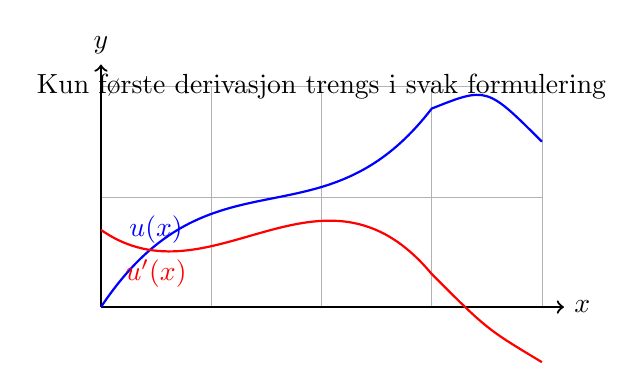
\begin{tikzpicture}[scale=1.4]
        % Grid and axes
        \draw[step=1.0, very thin, black!30] (0,0) grid (4,2);
        \draw[->,thick] (0,0) -- (4.2,0) node[right] {$x$};
        \draw[->,thick] (0,0) -- (0,2.2) node[above] {$y$};

        % Original function u(x)
        \draw[blue, thick] (0,0) .. controls (1,1.5) and (2,0.5) .. (3,1.8) .. controls (3.5,2) .. (4,1.5);

        % First derivative u'(x)
        \draw[red, thick] (0,0.7) .. controls (1,0) and (2,1.5) .. (3,0.3) .. controls (3.5,-0.2) .. (4,-0.5);

        % Labels
        \node[blue] at (0.5,0.7) {$u(x)$};
        \node[red] at (0.5,0.3) {$u'(x)$};
        \node[black] at (2,2) {Kun første derivasjon trengs i svak formulering};
    \end{tikzpicture}
    \caption{I svak formulering trenger vi bare første deriverte av $u(x)$}
    \label{fig:weak_formulation_derivative}
\end{figure}


\begin{figure}[H]
    \centering
    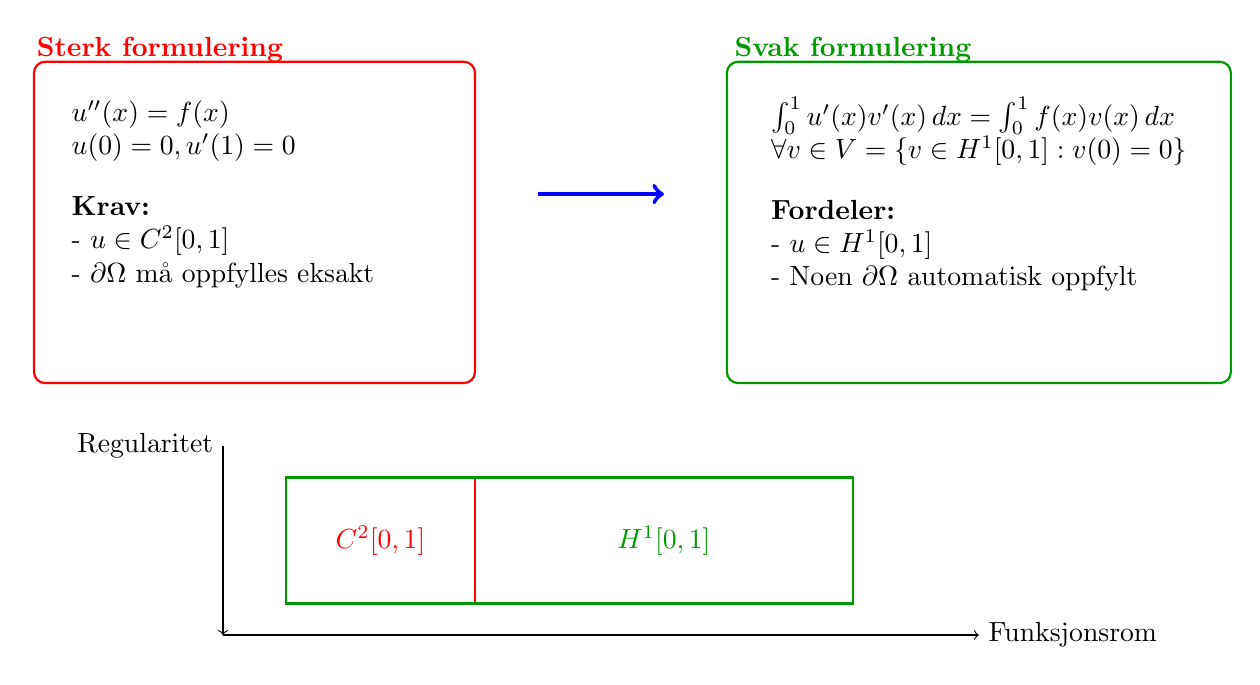
\begin{tikzpicture}[scale=0.8]
        % Box for strong formulation
        \draw[red, thick, rounded corners] (-1,0) rectangle (6,5.1);
        \node[red, font=\bfseries] at (1,5.3) {Sterk formulering};

        % Content of strong formulation
        \node[align=left] at (2,3) {
        $u^{\prime\prime}(x) = f(x)$ \\
        $u(0) = 0, u'(1) = 0$ \\[1em]
        \textbf{Krav:} \\
        - $u \in C^2[0,1]$ \\
        - $\partial \Omega$ må oppfylles eksakt
        };
        % Arrow and transformation label
        \draw[blue, ultra thick, ->] (7,3) -- (9,3);
        % Box for weak formulation
        \draw[green!60!black, thick, rounded corners] (10,0) rectangle (18,5.1);
        \node[green!60!black, font=\bfseries] at (12,5.3) {Svak formulering};
        % Content of weak formulation
        \node[align=left] at (14, 3) {
        $\int_0^1 u'(x)v'(x) \,dx = \int_0^1 f(x)v(x) \,dx$ \\
        $\forall v \in V = \{v \in H^1[0,1] : v(0) = 0\}$ \\[1em]
        \textbf{Fordeler:} \\
        - $u \in H^1[0,1]$  \\
        - Noen $\partial \Omega$ automatisk oppfylt
        };

        % Function spaces comparison
        \draw[->] (2,-1) -- (2,-4);
        \draw[->] (2,-4) -- (14,-4);
        \node[left] at (2,-1) {Regularitet};
        \node[right] at (14,-4) {Funksjonsrom};

        % Function spaces
        \draw[red, thick] (3,-1.5) rectangle (6,-3.5);
        \node[red] at (4.5,-2.5) {$C^2[0,1]$};

        \draw[green!60!black, thick] (3,-1.5) rectangle (12,-3.5);
        \node[green!60!black] at (9,-2.5) {$H^1[0,1]$};
    \end{tikzpicture}
    \caption{Sammenligning av sterk og svak formulering av differensialligninger}
    \label{fig:formulation_comparison}
\end{figure}

\subsection{Sammenheng med FEM}

Den svake formuleringen er grunnlaget for endelig element-metoden (FEM).
I FEM antar vi at:

\begin{align*}
    u(x) & \approx \sum_{i=1}^n c_i \varphi_i(x)        \\
    v(x) & = \varphi_j(x) \quad \text{for } j=1,2,...,n
\end{align*}

hvor $\varphi_i(x)$ er basisfunksjoner (typisk stykkevis lineære funksjoner). Ved å sette disse uttrykkene inn i den svake formuleringen, får vi et lineært ligningssystem for koeffisientene $c_i$:

\begin{align*}
    \sum_{i=1}^n c_i \int_0^1 \varphi_i^{\prime}(x) \varphi_j^{\prime}(x) \, dx & = \int_0^1 f(x) \varphi_j(x) \, dx \quad \text{for } j=1,2,...,n
\end{align*}

Dette kan skrives på matriseform som:

\begin{align*}
    \mathbf{K} \mathbf{c} = \mathbf{F}
\end{align*}

hvor:
\begin{align*}
    K_{ji} & = \int_0^1 \varphi_i^{\prime}(x) \varphi_j^{\prime}(x) \, dx \\
    F_j    & = \int_0^1 f(x) \varphi_j(x) \, dx
\end{align*}

Denne formuleringen er grunnlaget for numerisk løsning av differensialligninger ved hjelp av endelig element-metoden.

\begin{figure}[H]
    \centering
    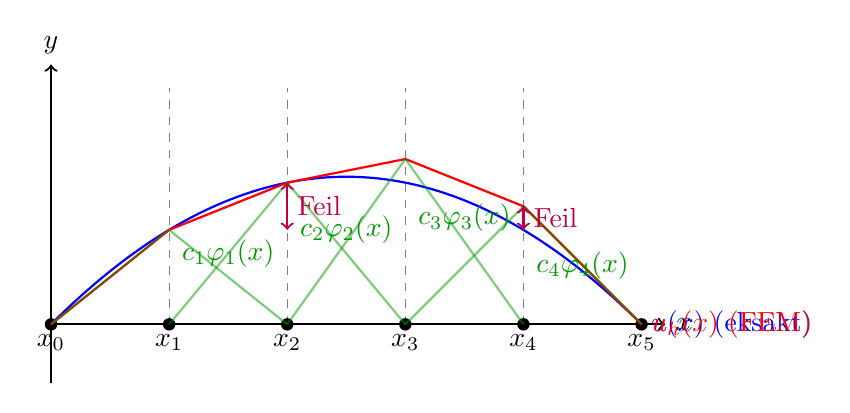
\begin{tikzpicture}[scale=1.5]
        % Axes
        \draw[->,thick] (0,0) -- (5.2,0) node[right] {$x$};
        \draw[->,thick] (0,-0.5) -- (0,2.2) node[above] {$y$};

        % Grid
        \foreach \x in {1,2,3,4}
        \draw[dashed,gray] (\x,0) -- (\x,2);

        % Node points
        \foreach \x in {0,1,2,3,4,5}
        \fill (\x,0) circle (1.5pt) node[below] {$x_{\x}$};

        % True solution
        \draw[thick, blue, domain=0:5, samples=100]
        plot (\x, {0.2*\x*(5-\x)});
        \node[blue, right] at (5, 0) {$u(x)$ (eksakt)};

        % FEM solution
        \draw[thick, red] (0,0) -- (1,0.8) -- (2,1.2) -- (3,1.4) -- (4,1.0) -- (5,0);
        \node[red, right] at (5, 0) {$u_h(x)$ (FEM)};

        % Basis functions - scaled by coefficients
        \draw[green!60!black, thick, opacity=0.5] (0,0) -- (1,0.8) -- (2,0);
        \draw[green!60!black, thick, opacity=0.5] (1,0) -- (2,1.2) -- (3,0);
        \draw[green!60!black, thick, opacity=0.5] (2,0) -- (3,1.4) -- (4,0);
        \draw[green!60!black, thick, opacity=0.5] (3,0) -- (4,1.0) -- (5,0);

        \node[green!60!black] at (1.5, 0.6) {$c_1\varphi_1(x)$};
        \node[green!60!black] at (2.5, 0.8) {$c_2\varphi_2(x)$};
        \node[green!60!black] at (3.5, 0.9) {$c_3\varphi_3(x)$};
        \node[green!60!black] at (4.5, 0.5) {$c_4\varphi_4(x)$};

        % Error indication
        \draw[<->,purple,thick] (2,1.2) -- (2,0.8) node[midway,right] {Feil};
        \draw[<->,purple,thick] (4,1.0) -- (4,0.8) node[midway,right] {Feil};
    \end{tikzpicture}
    \caption{FEM-løsning ($u_h(x)$) som en sum av vektede basisfunksjoner, sammenlignet med den eksakte løsningen ($u(x)$)}
    \label{fig:fem_solution}
\end{figure}

\begin{figure}[H]
    \centering
    \begin{tikzpicture}[scale=1.5, transform shape]
        % Axes
        \draw[->,thick] (0,0) -- (2.2,0) node[right] {$x$};
        \draw[->,thick] (0,0) -- (0,1.2) node[above] {$y$};

        % Mesh points
        \foreach \x in {0,0.5,1,1.5,2}
        \fill (\x,0) circle (0.5pt) node[below=1pt] {$\x$};

        % System matrix visualization
        \matrix [matrix of nodes, nodes={minimum size=6mm},
        row sep=-\pgflinewidth, column sep=-\pgflinewidth,
        draw=black, thick, outer sep=0pt, anchor=north west] (K) at (2.5,1) {
        |[fill=red!20]| $2$ & |[fill=red!15]| $-1$ & |[fill=red!5]| $0$ & |[fill=red!5]| $0$ \\
        |[fill=red!15]| $-1$ & |[fill=red!20]| $2$ & |[fill=red!15]| $-1$ & |[fill=red!5]| $0$ \\
        |[fill=red!5]| $0$ & |[fill=red!15]| $-1$ & |[fill=red!20]| $2$ & |[fill=red!15]| $-1$ \\
        |[fill=red!5]| $0$ & |[fill=red!5]| $0$ & |[fill=red!15]| $-1$ & |[fill=red!20]| $2$ \\
        };
        \node[above=1mm] at (K.north) {$\mathbf{K}$ (stivhetsmatrise)};

        % Solution vector
        \matrix [matrix of nodes, nodes={minimum size=6mm},
        row sep=-\pgflinewidth, column sep=-\pgflinewidth,
        draw=black, thick, outer sep=0pt,
        anchor=north west] (u) at (4.0,1) {
        |[fill=blue!20]| $c_1$ \\
        |[fill=blue!20]| $c_2$ \\
        |[fill=blue!20]| $c_3$ \\
        |[fill=blue!20]| $c_4$ \\
        };
        \node[above=1mm] at (u.north) {$\mathbf{c}$};

        % Equals sign
        \node at (4.5,0.45) {$=$};

        % Right-hand side vector
        \matrix [matrix of nodes, nodes={minimum size=6mm},
        row sep=-\pgflinewidth, column sep=-\pgflinewidth,
        draw=black, thick, outer sep=0pt,
        anchor=north west] (f) at (5.0,1) {
        |[fill=green!15]| $F_1$ \\
        |[fill=green!15]| $F_2$ \\
        |[fill=green!15]| $F_3$ \\
        |[fill=green!15]| $F_4$ \\
        };
        \node[above=1mm] at (f.north) {$\mathbf{F}$};

        % Example basis functions
        \draw[thick, blue] (0,0) -- (0.5,1) -- (1,0);
        \draw[thick, red] (0.5,0) -- (1,1) -- (1.5,0);
        \draw[thick, green!60!black] (1,0) -- (1.5,1) -- (2,0);

        % Labels
        \node[blue, scale=0.8] at (0.4,0.6) {$\varphi_1(x)$};
        \node[red, scale=0.8] at (0.9,0.6) {$\varphi_2(x)$};
        \node[green!60!black, scale=0.8] at (1.5,0.6) {$\varphi_3(x)$};
    \end{tikzpicture}
    \caption{FEM diskretisering: basisfunksjoner $\varphi_i(x)$ og tilhørende ligningssystem $\mathbf{K}\mathbf{c} = \mathbf{F}$}
    \label{fig:fem_discretization}
\end{figure}


Her skriver vi pde direkte i differensialform.
Det betyr at vi forutsetter at løsningen \(u(x)\) er glatt nok til at alle deriverte eksisterer.
Da har vi:
\[
    \mathcal{L}(u) = f,
\]
samt presise krav på grenseverdier, for eksempel:
\[
    u|_{\partial \Omega} = g \quad \text{eller} \quad \frac{\partial u}{\partial n}\bigg|_{\partial \Omega} = h.
\]

Hvis løsningen u ikke er glatt nok, bruker vi en weakformulation av problemet.

\section{Svak form}

Her tester vi u med en testfunksjon \(v(x)\) over hele domenet:
\[
    \int_\Omega v^{(k)}(x) \, \mathcal{L}(u(x)) \, dx = \int_\Omega v(x) \, f(x) \, dx.
\]
Denne metoden gjør det mulig å finne løsninger i et bredere funksjonsrom.

testfunksjon er en vilkårlig funksjon som tilfredsstiller randbetingelsene, og velges ofte til å være det samme som basisfunction:
\[
    v(x) = \sum_{j=1}^n v_j \phi_j(x) = \symbf{v}^T \symbf{\phi}(x)
\]


\subsection{Fra sterk form}
Her skriver vi pde-en direkte i differensialform. Det betyr at vi forutsetter at løsningen u er glatt nok til at alle deriverte eksisterer. Da har vi:
\[
    \mathcal{L}(u) = f,
\]
samt presise krav på grenseverdier, for eksempel:
\[
    u|_{\partial \Omega} = g \quad \text{eller} \quad \frac{\partial u}{\partial n}\bigg|_{\partial \Omega} = h.
\]

\subsection{Til svak form}
For løsninger som ikke er tilstrekkelig glatte, bruker vi en weakformulation:

\begin{enumerate}
    \item Multipliser PDE-en med en testfunksjon $v(x)$
    \item Integrer over domenet $\Omega$:
          \[
              \int_\Omega v^{(k)}(x) \, \mathcal{L}(u(x)) \, dx = \int_\Omega v(x) \, f(x) \, dx
          \]
\end{enumerate}

\subsection{Fordeler med svak form}
\begin{itemize}
    \item Tillater løsninger i bredere funksjonsrom
    \item Reduserer glatthetskrav
    \item Gir mer fleksible randbetingelser
\end{itemize}

En testfunksjon $v(x)$ tilfredsstiller randbetingelsene og uttrykkes i Galerkin-metoden ved:
\[
    v(x) = \sum_{j=1}^n v_j \phi_j(x) = \symbf{v}^T \symbf{\phi}(x)
\]

\section{Basisfunksjoner (Formfunksjoner)}

Basisfunksjoner er byggesteinene i fem-metoden.
De er enkle funksjoner som gjør at vi kan representere en komplisert funksjon ved hjelp av enkle byggesteiner.

En basisfunction \(\phi_i(x)\) er en lokal funksjon som:
\begin{itemize}
    \item Er null overalt unntatt i nærheten av node \(i\) (lokalt definert).
    \item Har verdien 1 i node \(i\) og 0 i alle andre noder
    \item Til sammen kan bygge opp løsningen vår \(u(x)\) som en sum:
          \[
              u(x) = \sum_{i=1}^n u_i \phi_i(x) = \symbf{u}^T \symbf{\phi}(x)
          \]
    \item \(u_i\) er koeffisientene som bestemmer hvor mye av hver basisfunction som skal brukes.
\end{itemize}


\subsection{Stykkvis lineære basisfunksjoner}

La \(u(x)\) være en tilnærming til løsningen av et pde, og la \(u(x)\) være gitt ved en lineærkombinasjon av basisfunctioner:
\[
    u(x) = \sum_{i=1}^6 u_i N_i(x)
\]

\begin{figure}[H]
    \centering
    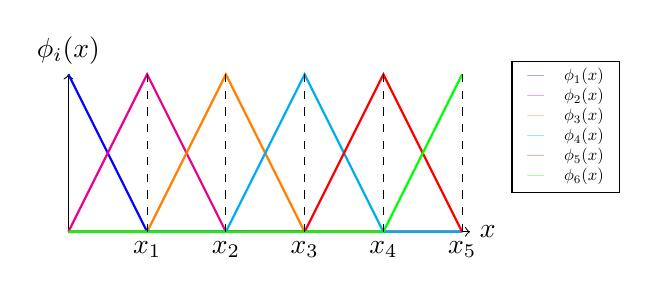
\begin{tikzpicture}
        % Coordinate axes
        \draw[->] (0,0) -- (0,2) node[above] {\(\phi_i(x)\)};
        \draw[->] (0,0) -- (5.1,0) node[right] {\(x\)};

        % Solution curve
        \draw[thick, blue] (0,2) -- (1,0) -- (5,0);
        \draw[thick, magenta] (0,0) -- (1,2) -- (2,0) -- (5,0);
        \draw[thick, orange] (0,0) -- (1,0) -- (2,2) -- (3,0) -- (5,0);
        \draw[thick, cyan] (0,0) -- (2,0) -- (3,2) -- (4,0) -- (5,0);
        \draw[thick, red] (0,0) -- (3,0) -- (4,2) -- (5,0);
        \draw[thick, green] (0,0) -- (4,0) -- (5,2);

        % Vertical lines at nodes with labels
        \draw[dashed] (1,0) node[below] {\(x_1\)} -- (1,2);
        \draw[dashed] (2,0) node[below] {\(x_2\)} -- (2,2);
        \draw[dashed] (3,0) node[below] {\(x_3\)} -- (3,2);
        \draw[dashed] (4,0) node[below] {\(x_4\)} -- (4,2);
        \draw[dashed] (5,0) node[below] {\(x_5\)} -- (5,2);

        % Legend
        \node[draw, anchor=south east, scale=0.6,fill=white] at (7,0.5) {
            \begin{tabular}{ll}
                \textcolor{blue}{---}    & \(\phi_1(x)\) \\
                \textcolor{magenta}{---} & \(\phi_2(x)\) \\
                \textcolor{orange}{---}  & \(\phi_3(x)\) \\
                \textcolor{cyan}{---}    & \(\phi_4(x)\) \\
                \textcolor{red}{---}     & \(\phi_5(x)\) \\
                \textcolor{green}{---}   & \(\phi_6(x)\) \\
            \end{tabular}
        };

    \end{tikzpicture}
    \caption{Piecewise Linear Basis Functions \(\phi_i(x)\)}
\end{figure}

\subparagraph{FEM for Poisson-ligningen}
\begin{equation}
    \begin{cases}
        -\ddn[2]{u(x)}{x} = f(x),         & x \in (0,1)              \\
        u(0) = \alpha, \quad u(1) = \beta & \text{(randbetingelser)}
    \end{cases}
    \label{eq:pde_poisson}
\end{equation}

\begin{equation}
    \mathbf{F} = - \int_0^1 f(x) \mathbf{N}(x) dx
\end{equation}

La \(f(x) = \bar{f} = C\) være konstant.

Vi antar at \(u(x_m)\) er ukjent for \(m = 1, \ldots, M\) punkter (noder) i det diskrete domainet \(\Omega_h\).

I mellom nodene definerer vi \textit{elementene} \(\implies\) \textit{formfunksjoner} \(N_i(x)\).
\begin{example}{}{}
    \begin{itemize}
        \item \textbf{Eksakt løsning:} $u$
        \item \textbf{Numerisk løsning:} $u_h$
        \item \textbf{Feil:} $e = \norm*{u - u_h}$
    \end{itemize}

    La $\norm*{u - v}_{\mathcal{H}^1}$ for en tilfeldig $v \in \mathcal{X}_h^1$.

    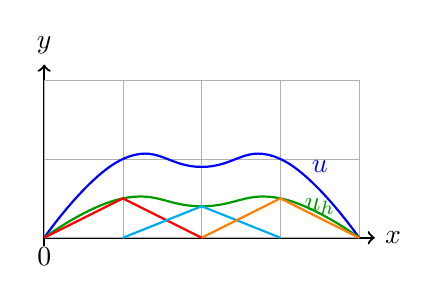
\begin{tikzpicture}
        % Axes
        \draw[->,thick] (0,0) -- (4.2,0) node[right] {$x$};
        \draw[->,thick] (0,0) -- (0,2.2) node[above] {$y$};

        % Grid
        \draw[step=1.0, very thin, black!30] (0,0) grid (4,2);
        \draw[thick] (0,-0.1) -- (0,0) node[below] {$0$};

        % Exact solution u(x) (curve looking like two small hills)
        \draw[blue, thick, smooth, tension=0.8] plot coordinates {(0,0) (1,1) (2,0.9) (3,1) (4,0)};
        \node[blue] at (3.5,0.9) {$u$};
        \draw[green!60!black, thick, smooth, tension=0.8] plot coordinates {(0,0) (1,0.5) (2,0.4) (3,0.5) (4,0)};
        \node[green!60!black] at (3.5,0.4) {$u_h$};


        % Basis functions
        \draw[thick, red] (0,0) -- (1,0.5) -- (2,0);
        \draw[thick, cyan] (1,0) -- (2,0.4) -- (3,0);
        \draw[thick, orange] (2,0) -- (3,0.5) -- (4,0);

    \end{tikzpicture}
\end{example}

\section{Interpolasjonsoperator}
\label{sec:interpolasjonsoperator}
Vi definerer en interpolasjonsoperator $\Pi_h^1: \mathbb{H}(\Omega)^1 \to \mathbb{X}_h^1$.
\begin{align*}
    \Pi_h^1 v(x_i) & = v(x_i) \quad i = 0, 1, \ldots, M                          \\
    \Pi_h^1 v(x)   & = \sum_{i=0}^M v(x_i) \varphi_i(x) \in \mathbb{X}_h^1 = V_h
\end{align*}

Med interpolasjonsfeilen:
\[
    e(x) = v(x) - \Pi_h^1 v(x)
\]
som vi ønsker å finne en øvre grense for \(\norm*{e(x)}_{\mathbb{H}^1} \).

La nå $H^2(\Omega) = \{v \in H^1(\Omega) : v_{xx} \in L^2(\Omega)\}$ være et Hilbert-rom med norm $\abs*{v}_{H^2}^2 = \int_\Omega v_{xx}^2 \, dx$.

\begin{align*}
    \norm*{e(x)}_{\mathbb{H}^1} & = \int_0^1 e^2 \, dx + \int_0^1 e_x^2 \, dx                                                   \\
                                & = \sum_{k\in\mathcal{T}_h} \int_{k} e^2 \, dx + \sum_{k\in\mathcal{T}_h} \int_{k} e_x^2 \, dx
\end{align*}

Vi vet at $e(x_k) = e(x_{k+1}) = 0$.

For $x > \xi_k$:

\begin{align*}
    e_x(x) = \int_{\xi_k}^x e_{xx} \, ds = \int_{\xi_k}^x v_{xx} \, ds
\end{align*}

Fordi $(\Pi_h^1 v)_{xx} = 0$.

For $x < \xi_k$:
\begin{align*}
    e_x(x)                                           & =-\int_{x}^{\xi_k} v_{xx} \, ds                                                                                                                                                \\
    \abs*{e_x}_K \leq \int_{K_k} \abs*{v_{xx}} \, dx & = \int_{K_k} 1\cdot \abs*{v_{xx}} \, dx                                                                                                                                        \\
                                                     & = \inner{1, \abs*{v_{xx}}}_{L^2(K_k)} \leq \norm*{1}_{L^2(K_k)} \norm*{\abs*{v_{xx}}}_{L^2(K_k)} \tag{Cauchy-Schwarz}                                                          \\
    \abs*{e_x}_{K_k}                                 & \leq \underbrace{\sqrt{\int_{K_k} 1^2 \, ds}}_{h_k} \times \sqrt{\int_{K_k} v_{xx}^2 \, ds} \quad \text{hvor } h_k = x_{k+1} - x_k                                             \\
    \abs*{e_x}_{K_k}^2                               & \leq h_k \int_{K_k} v_{xx}^2 \, ds                                                                                                                                             \\
    h                                                & = \max_{k \in \mathcal{T}_h} h_k                                                                                                                                               \\
    \abs*{e}_{H^1(K)}^2                              & = \int_{K_k} e_x^2 \, dx \leq h_k^2 \int_{K_k} v_{xx}^2 \, dx                                                                                                                  \\
    \abs*{e}_{H^1(\Omega)}^2                         & = \sum_{k\in\mathcal{T}_h} \abs*{e_x}_{H^1(K)}^2 \leq h^2 \sum_{k\in\mathcal{T}_h} \int_{K_k} v_{xx}^2 \, dx = h^2 \int_{\Omega} v_{xx}^2 \, dx = h^2 \abs*{v}_{H^2(\Omega)}^2 \\
    \norm*{e}_{\mathcal{L}^2(\Omega)}                & \leq h^4 \abs*{v}_{H^2(\Omega)}^2                                                                                                                                              \\
    \norm*{e}_{H^1(\Omega)}                          & = \norm*{e}_{\mathcal{L}^2(\Omega)} + \abs*{e}_{H^1(\Omega)} \leq (h^4 + h^2) \abs*{v}_{H^2(\Omega)}^2 \leq K^2 h^2 \norm*{v}_{H^2(\Omega)}^2                                  \\
\end{align*}

Hvis vi bruker Ceas lemma med $v = \Pi_h^1(u)$, får vi:

\begin{align*}
    \norm*{u - u_h}_{H^1(\Omega)} & \leq \frac{M}{\alpha} \abs*{u}_{H^2(\Omega)} h \leq C \abs*{u}_{H^2(\Omega)} h
\end{align*}
Er en første ordens metode. Fungerer kun hvis $u \in H^2(\Omega)$.

\subsection{Modell problem}

\begin{align*}
    -\Delta u(x) & = f(x) \quad x \in \Omega      \\
    u(x)         & = 0 \quad x \in \partial\Omega
\end{align*}
\begin{itemize}
    \item Hva er den svake formuleringen av dette problemet?
    \item Er LM-teoremet oppfylt?
    \item Hva er $X_h^1$ i dette tilfellet?
\end{itemize}
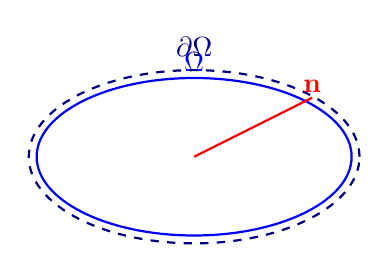
\begin{tikzpicture}
    % Omega ellipse
    \draw[thick, blue] (0,0) ellipse (2 and 1);
    \node[blue] at (0,1.2) {$\Omega$};
    % Boundary
    \draw[thick, dashed, blue!50!black] (0,0) ellipse (2.1 and 1.1);
    \node[blue!50!black] at (0,1.4) {$\partial\Omega$};

    % Normalvector
    \draw[thick, red] (0,0) -- (1.5,0.75);
    \node[red] at (1.5,0.9) {$\mathbf{n}$};

\end{tikzpicture}

\begin{itemize}
    \item $\Omega$ er en åpen, begrenset og sammenhengende delmengde.
    \item $\partial\Omega$ er den lukkede mengden av alle punkter i $\Omega$.
    \item $\overline{\Omega} = \Omega \cup \partial\Omega$ er den lukkede mengden av alle punkter i $\Omega$.
    \item $v: \Omega \to \mathbb{R}$
    \item $\mathbf{F}: \Omega \to \mathbb{R}^2$
\end{itemize}
\paragraph{Vektor notasjon}
\subparagraph{Gradient}
\begin{align*}
    \nabla u(x) & = \begin{pmatrix}
                        \frac{\partial u}{\partial x_1} \\
                        \frac{\partial u}{\partial x_2}
                    \end{pmatrix} = \begin{pmatrix}
                                        u_{x_1} \\
                                        u_{x_2}
                                    \end{pmatrix} = (u_{x_1}, u_{x_2})^T
\end{align*}
\subparagraph{Divergens}
\begin{align*}
    \nabla \cdot \mathbf{F} & = \frac{\partial F_1}{\partial x_1} + \frac{\partial F_2}{\partial x_2} = F_{x_1} + F_{x_2}
\end{align*}

\subparagraph{Laplace operator}
\begin{align*}
    \Delta u(x) & = \nabla^2 u(x) = \nabla \cdot \nabla u(x) = \frac{\partial^2 u}{\partial x_1^2} + \frac{\partial^2 u}{\partial x_2^2} = u_{x_1x_1} + u_{x_2x_2}
\end{align*}

\begin{theorem}{Divergensteoremet}{divergence_theorem}
    \[
        \int_{\Omega} \nabla \cdot \mathbf{F} \, dx = \int_{\partial\Omega} \mathbf{F} \cdot \mathbf{n} \, ds
    \]
    \begin{itemize}
        \item $\mathbf{F}$ er en vektorfelt.
        \item $\mathbf{n}$ er en normalvektor til grensen $\partial\Omega$.
        \item $ds$ er et infinitesimalt areal på grensen $\partial\Omega$.
        \item $dx$ er et infinitesimalt areal i domenet $\Omega$.
        \item $\int_{\partial\Omega} \mathbf{F} \cdot \mathbf{n} \, ds$ er fluks gjennom grensen $\partial\Omega$.
        \item $\int_{\Omega} \nabla \cdot \mathbf{F} \, dx$ er divergensen av vektorfeltet $\mathbf{F}$ i domenet $\Omega$.
    \end{itemize}
\end{theorem}


\subparagraph{Laplace operator}
\begin{align*}
    \Delta u(x) & = \nabla^2 u(x) = \nabla \cdot \nabla u(x) = \frac{\partial^2 u}{\partial x_1^2} + \frac{\partial^2 u}{\partial x_2^2} = u_{x_1x_1} + u_{x_2x_2}
\end{align*}

\subparagraph{Vektor Kalkulus}
\begin{align*}
    \nabla \cdot (v \mathbf{F}) & = \nabla v \cdot \mathbf{F} + v \nabla \cdot \mathbf{F} \\
\end{align*}

\subparagraph{Green's teorem}
La $u: \Omega \to \mathbb{R}$ og $\mathbf{F} = \nabla u$ være en vektorfelt. Da har vi at:

\begin{align*}
    \int_{\Omega} \nabla v \cdot \nabla u \, d\Omega + \int_{\Omega} v \Delta u \, d\Omega & = \oint_{\partial\Omega} v \nabla u \cdot \mathbf{n} \, d\gamma
\end{align*}

$-\Delta u = f$ på $\Omega$ og $u = 0$ på $\partial\Omega$ gir oss:
\begin{align*}
    \int_{\Omega} \nabla v \cdot \nabla u \, d\Omega & = \oint_{\partial\Omega} v \nabla u \cdot \mathbf{n} \, d\gamma
\end{align*}
Krever at $v = 0$ på $\partial\Omega$.

Definerer:
\begin{align*}
    H^1(\Omega)                & = \{v: \Omega \to \mathbb{R}, v, v_{x_1}, v_{x_2} \in L^2(\Omega)\}                            \\
    L^2(\Omega)                & = \{v: \int_{\Omega} v^2 \, dx < \infty\}                                                      \\
    \inner{u, v}_{L^2(\Omega)} & = \int_{\Omega} u v \, d\Omega, \quad \norm*{v}_{L^2(\Omega)}^2 = \int_{\Omega} v^2 \, d\Omega \\
    H_0^1(\Omega)              & = \{v \in H^1(\Omega), v = 0 \text{ på } \partial\Omega\}
\end{align*}
\paragraph{Variasjonsformulering (Variational form)}
Finn $u \in H_0^1(\Omega)$ slik at $\int_{\Omega} \nabla u \cdot \nabla v \, d\Omega = \int_{\Omega} f v \, d\Omega$ for alle $v \in H_0^1(\Omega)$.
\begin{align*}
    V = H_0^1(\Omega) \\
    a(u, v) = \int_{\Omega} \nabla u \cdot \nabla v \, d\Omega, \quad F(v) = \int_{\Omega} f v \, d\Omega
\end{align*}


\begin{example}{Poisson}{poisson-1}
    \paragraph{Sterk form}
    Finn $u: \Omega \to \mathbb{R}$ slik at
    \begin{align*}
        -\Delta u & = f \quad \text{i } \Omega,          \\
        u         & = 0 \quad \text{på } \partial\Omega,
    \end{align*}

    \paragraph{Svak form}
    Finn $u \in V$ slik at
    \begin{align*}
        \inner*{\nabla u, \nabla \phi} & = \inner*{f, \phi} \quad \forall \phi \in V := H^1_0(\Omega) = \{ u \in H^1(\Omega) : u = 0 \text{ på } \partial\Omega \}
    \end{align*}

    \paragraph{Diskret svak form}
    Finn $u_h \in V_h \subset V$ slik at
    \begin{align*}
        \inner*{\nabla u_h, \nabla \phi_i} & = \inner*{f, \phi_i} \quad \forall i = 1, \ldots, n,
    \end{align*}

    \paragraph{Løsning}
    Løs det lineære systemet $A\vec{u} = \vec{f}$, der
    \begin{align*}
        \inner*{\nabla u_h, \nabla \phi_i} & = \inner*{f, \phi_i},  \quad \Leftrightarrow \quad A\vec{u} = \vec{f}                          \\
        A_{ij}                             & = \inner*{\nabla \phi_j, \nabla \phi_i}, \quad \vec{u}_i, \quad \vec{f}_i = \inner*{f, \phi_i} \\
    \end{align*}

\end{example}

\subsection{Ekvivalente former}
\subsection*{Sterk form}
Finn $u \in \mathcal{C}^2(\Omega)$ slik at
\begin{align*}
    -u^{\prime\prime} & = f \quad \text{i } \Omega,          \\
    u                 & = 0 \quad \text{på } \partial\Omega,
\end{align*}

\subsection*{Svak form}
Finn $u \in V = H^1_0(\Omega)$ slik at
\begin{align*}
    \inner*{u^{\prime}, \phi^{\prime}} & = \inner*{f, \phi} \quad \forall \phi \in V := H^1_0(\Omega)
\end{align*}

\subsection*{Energiminimeringsform}
La $F: V \to \mathbb{R}$ være en energifunksjon definert som
\begin{align*}
    F(u) = \frac{1}{2} \inner*{u^{\prime}, u^{\prime}} - \inner*{f, u}
\end{align*}
Der $F(u)$ representerer energien i systemet. Den første termen representerer den kinetiske energien, mens den andre termen representerer den potensielle energien.

Finn $u \in V$ slik at
\begin{align*}
    F(u) \leq F(\phi) \quad \forall \phi \in V
\end{align*}

Dette er en variabel minimeringsoppgave der vi ønsker å finne den funksjonen $u$ som minimerer energien i systemet.\footnote{Det er ikke alltid at denne formen eksisterer for problemet vårt.}

\section{Eksempler}

\subsection{Poisson-ligningen}

\begin{example}{Poisson-ligningen}{poisson-2}
    Poisson-ligningen er en vanlig pde som beskriver mange fysiske fenomener, inkludert varmeledning og elektrisk potensial.
    Den kan skrives som:
    \begin{equation}
        \begin{cases}
            -\Delta u(x) = f(x),              & x \in (0,1)              \\
            u(0) = \alpha, \quad u(1) = \beta & \text{(randbetingelser)}
        \end{cases}
    \end{equation}

    \begin{equation}
        \mathbf{F} = - \int_0^1 f( x) \mathbf{N}(x) dx
    \end{equation}

    \begin{equation}
        \begin{cases}
            -\ddn[u]{2}{x} = f(x),            & x \in (0,1)              \\
            u(0) = \alpha, \quad u(1) = \beta & \text{(randbetingelser)}
        \end{cases}
    \end{equation}

\end{example}

La \(f(x) = \bar{f}\) være konstant. Vi antar at \(u(x_m)\) er ukjent for \(m = 1, \ldots, M\) punkter (noder) i det diskrete domenet \(\Omega_h\).

I mellom nodene definerer vi \textit{elementene} \(\implies\) \textit{formfunksjoner} \(N_i(x)\).

\begin{figure}[H]
    \centering
    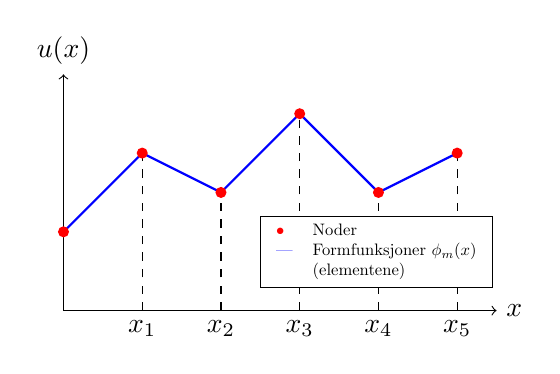
\begin{tikzpicture}
        % Coordinate axes
        \draw[->] (0,0) -- (0,3) node[above] {\(u(x)\)};
        \draw[->] (0,0) -- (5.5,0) node[right] {\(x\)};

        % Solution curve
        \draw[thick, blue] (0,1) -- (1,2) -- (2,1.5) -- (3,2.5) -- (4,1.5) -- (5,2);

        % Vertical lines at nodes with labels
        \draw[dashed] (1,0) node[below] {\(x_1\)} -- (1,2);
        \draw[dashed] (2,0) node[below] {\(x_2\)} -- (2,1.5);
        \draw[dashed] (3,0) node[below] {\(x_3\)} -- (3,2.5);
        \draw[dashed] (4,0) node[below] {\(x_4\)} -- (4,1.5);
        \draw[dashed] (5,0) node[below] {\(x_5\)} -- (5,2);

        % Nodes (intersection points)
        \fill[red] (0,1) circle (2pt);
        \fill[red] (1,2) circle (2pt);
        \fill[red] (2,1.5) circle (2pt);
        \fill[red] (3,2.5) circle (2pt);
        \fill[red] (4,1.5) circle (2pt);
        \fill[red] (5,2) circle (2pt);

        % Add legend
        \node[draw, anchor=north west, scale=0.6,fill=white] at (2.5,1.2) {
            \begin{tabular}{ll}
                \textcolor{red}{\(\bullet\)} & Noder                        \\
                \textcolor{blue}{---}        & Formfunksjoner \(\phi_m(x)\) \\
                                             & (elementene)                 \\
            \end{tabular}
        };
    \end{tikzpicture}
    \caption{Tilfeldig valgt formfunksjoner \(N_i(x)\) mellom nodene \(x_i\).}
\end{figure}
Definerer formfunksjonene som:
\[
    \phi_i(x) = \begin{cases}
        1 - 2|x - x_i|, & |x - x_i| < 0.5 \\
        0,              & \text{ellers}
    \end{cases}
\]
Og testfunksjonene som:
\[
    v(x) = \sum_{j=1}^n v_j \phi_j(x) = \symbf{v}^T \symbf{\phi}(x)
\]

Den svake formuleringen blir:
\begin{align*}
    \int_0^1 \left( \sum_{j=1}^n v_j \phi_j'(x) \right)
    \left( \sum_{i=1}^n u_i \phi_i'(x) \right) \, dx
                        & =
    \int_0^1 \left( \sum_{j=1}^n v_j \phi_j(x) \right) f(x) \, dx \\
    \symbf{v}^T \, \int_0^1 \symbf{\phi}' \symbf{\phi}'^T \, dx \, \symbf{u}
                        & =
    \symbf{v}^T \int_0^1 - f(x) \symbf{\phi}  \, dx               \\
    \symbf{v}^T \symbf{K} \symbf{u}
                        & =
    \symbf{v}^T \symbf{F}                                         \\
    \symbf{K} \symbf{u} & = \symbf{F}
\end{align*}

Hvor:

\begin{align*}
    \symbf{K} & = \int_0^1 \symbf{\phi}' \symbf{\phi}'^T \, dx =
    \begin{bmatrix}
        1  & -1 & 0  & 0  & 0  & 0  \\
        -1 & 2  & -1 & 0  & 0  & 0  \\
        0  & -1 & 2  & -1 & 0  & 0  \\
        0  & 0  & -1 & 2  & -1 & 0  \\
        0  & 0  & 0  & -1 & 2  & -1 \\
        0  & 0  & 0  & 0  & -1 & 1  \\
    \end{bmatrix}                                  \\
    \symbf{F} & = - \bar{f} \int_0^1 \symbf{N}(x) dx
    = - \bar{f}
    \begin{bmatrix}
        0.1 \\ 0.2 \\ 0.2 \\ 0.2 \\ 0.2 \\ 0.1
    \end{bmatrix}
\end{align*}

Løser ligningssystemet for å finne koeffisientene \(u_i\):
\[
    \symbf{u} = \symbf{K}^{-1} \symbf{F}
\]

\subsection{Svak formulering av Poisson-ligningen}
Vi kan skrive den svake formuleringen som:
\[
    \int_0^1 v'(x) u'(x) \, dx = \int_0^1 v(x) f(x) \, dx,
\]

Velger basisfunctioner til å være:
\[
    \phi_i(x) = \begin{cases}
        1 - 2|x - x_i|, & |x - x_i| < 0.5 \\
        0,              & \text{ellers}
    \end{cases}
\]
Med testfunksjonene \(v(x) = \sum_{j=1}^n v_j \phi_j(x)\).

Da får vi:

\begin{align*}
    \int_0^1 \left( \sum_{j=1}^n v_j \phi_j'(x) \right) \left( \sum_{i=1}^n u_i \phi_i'(x) \right) \, dx
                        & =
    \int_0^1 \left( \sum_{j=1}^n v_j \phi_j(x) \right) f(x) \, dx \\
    \symbf{v}^T \, \int_0^1 \symbf{\phi}' \symbf{\phi}'^T \, dx \, \symbf{u}
                        & =
    \symbf{v}^T \int_0^1 - f(x) \symbf{\phi}  \, dx               \\
    \symbf{v}^T \symbf{K} \symbf{u}
                        & =
    \symbf{v}^T \symbf{F}                                         \\
    \symbf{K} \symbf{u} & = \symbf{F}
\end{align*}
\begin{figure}[H]
    \centering
    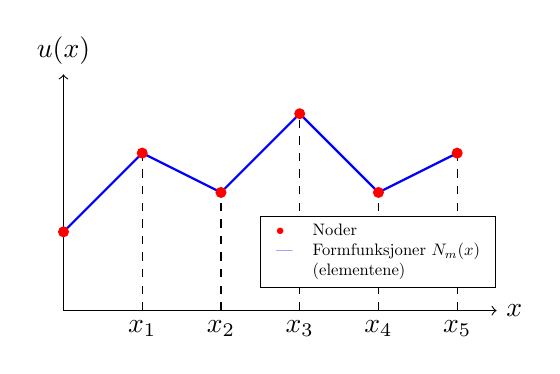
\begin{tikzpicture}
        % Coordinate axes
        \draw[->] (0,0) -- (0,3) node[above] {\(u(x)\)};
        \draw[->] (0,0) -- (5.5,0) node[right] {\(x\)};

        % Solution curve
        \draw[thick, blue] (0,1) -- (1,2) -- (2,1.5) -- (3,2.5) -- (4,1.5) -- (5,2);

        % Vertical lines at nodes with labels
        \draw[dashed] (1,0) node[below] {\(x_1\)} -- (1,2);
        \draw[dashed] (2,0) node[below] {\(x_2\)} -- (2,1.5);
        \draw[dashed] (3,0) node[below] {\(x_3\)} -- (3,2.5);
        \draw[dashed] (4,0) node[below] {\(x_4\)} -- (4,1.5);
        \draw[dashed] (5,0) node[below] {\(x_5\)} -- (5,2);

        % Nodes (intersection points)
        \fill[red] (0,1) circle (2pt);
        \fill[red] (1,2) circle (2pt);
        \fill[red] (2,1.5) circle (2pt);
        \fill[red] (3,2.5) circle (2pt);
        \fill[red] (4,1.5) circle (2pt);
        \fill[red] (5,2) circle (2pt);

        % Add legend
        \node[draw, anchor=north west, scale=0.6,fill=white] at (2.5,1.2) {
            \begin{tabular}{ll}
                \textcolor{red}{\(\bullet\)} & Noder                     \\
                \textcolor{blue}{---}        & Formfunksjoner \(N_m(x)\) \\
                                             & (elementene)              \\
            \end{tabular}
        };
    \end{tikzpicture}
    \caption{Tilfeldig valgt formfunksjoner \(N_i(x)\) mellom nodene \(x_i\).}
\end{figure}

\begin{equation*}
    \symbf{F} = - \bar{f} \int_0^1 \symbf{N}(x) dx = - \bar{f} \begin{bmatrix}
        0.1 \\ 0.2 \\ 0.2 \\ 0.2 \\ 0.2 \\ 0.1
    \end{bmatrix}
\end{equation*}


\begin{example}{Eksamen Vår 2024}{}
    Vi har ett en-dimesjonalt elliptisk randverdi-problem.
    \begin{equation*}
        -\mathcal{L}u  = -\frac{d}{dx} \left( (1 + x) \frac{du}{dx} \right) + 2u = 2x \quad x \in (0, 1) \quad
        u(0)           = \sqrt{2}, \quad u(1) = \sqrt{3}
        \label{eq:v2024_p4b}
    \end{equation*}
    La nå \(M \in \mathbb{N}\) og \(\Tau_h = \bigcup_{i=1}^M K_i\) være en triangulering av \((0, 1)\) med \(K_i = (x_{i-1}, x_i)\), \(x_i = ih\) og \(h = \frac{1}{M}\).

    \begin{align*}
        \Tau_h & = \{K_1, K_2, \ldots, K_M\}=\{(x_0, x_1), (x_1, x_2), \ldots, (x_{M-1}, x_M)\}
    \end{align*}

    Finn \textbf{elementmatrisen} $A^{K_i}$ og \textbf{lastvektoren} $\symbf{F}^{K_i}$ for Lagrange FEM i $\mathbb{P}_1$ på trianguleringen $\Tau_h$ for problemet i \eqref{eq:v2024_p4b}.

    På $\mathbb{P}_1$ er standard Lagrange-FEM-basisfunksjonene gitt ved:
    \begin{align*}
        \phi_1(x) & = \frac{x_i - x}{h}     & \phi_1(x_{i-1}) = 1, \phi_1(x_i) = 0 \\
        \phi_2(x) & = \frac{x - x_{i-1}}{h} & \phi_2(x_{i-1}) = 0, \phi_2(x_i) = 1
    \end{align*}

    Først finner vi testfunksjonene \(v \in \mathcal{H}_0^1(0, 1)\) og basisfunksjonene \(\phi_i(x)\) for \(i = 1, \ldots, M\).
    \begin{align*}
        v(x) & = \sum_{i=1}^M v_i \phi_i(x) \\
    \end{align*}
\end{example}

\subsection{Svak formulering}
Den svake formuleringen av problemet i \eqref{eq:v2024_p4b} finner man ved å gange PDE med testfunksjonen \(v\) på begge sidene og integrere over \((0, 1)\):
\begin{align*}
    -\int_0^1  \mathcal{L}u(x) v(x) \, dx                                                              & = 0                      \\
    \int_0^1  \left[-\frac{d}{dx} \left( (1 + x) \frac{du}{dx} \right) + 2u \right] v(x) \, dx         & = 2\int_0^1 x v(x) \, dx \\
    -\int_0^1 \frac{d}{dx} \left( (1 + x) u^{\prime}(x) \right) v(x) \, dx + 2\int_0^1 u(x) v(x) \, dx & = 2\int_0^1 x v(x) \, dx
\end{align*}

For det første leddet i LHS bruker vi delvis integrasjon:

\begin{align*}
    -\int_0^1 \overbrace{\frac{d}{dx} \left( (1 + x)u^{\prime}(x) \right)}^{w^\prime(x)} v(x) \, dx & = -\left[w(x)v(x)\right]_0^1 + \int_0^1 w(x)v^\prime(x) \, dx                                                        \\
                                                                                                    & = -\left[(1 + x)u^{\prime}(x)v(x)\right]_0^1 + \int_0^1 (1 + x)u^{\prime}(x)v^\prime(x) \, dx                        \\
                                                                                                    & = -\left[(1 + 1)u^{\prime}(1)v(1) - (1 + 0)u^{\prime}(0)v(0)\right] + \int_0^1 (1 + x)u^{\prime}(x)v^\prime(x) \, dx \\
                                                                                                    & = -\left[2u^{\prime}(1)v(1) - u^{\prime}(0)v(0)\right] + \int_0^1 (1 + x)u^{\prime}(x)v^\prime(x) \, dx              \\
                                                                                                    & = 0 + \int_0^1 (1 + x)u^{\prime}(x)v^\prime(x) \, dx
\end{align*}

Siden $v \in \mathcal{H}_0^1(0, 1)$, så er \(v(0) = v(1) = 0\) får vi at $[w(x)v(x)]_0^1 = 0$.

Dermed kan vi skrive om den svake formuleringen til:
\begin{align*}
    \int_0^1 (1 + x)u^{\prime}(x)v^\prime(x) \, dx + 2\int_0^1 u(x) v(x) \, dx & = 2\int_0^1 x v(x) \, dx \\
    \int_0^1 (1 + x)u^{\prime}(x)v^\prime(x) + 2u(x)v(x) \, dx                 & = 2\int_0^1 x v(x) \, dx
\end{align*}

Vi approksimerer \(u\) med Lagrange-FEM-basisfunksjoner \(\phi_i(x)\) i \(\mathbb{P}_1\):
\begin{align*}
    u(x) & \approx \sum_{i=1}^M u_i \phi_i(x) = \symbf{u}^T \symbf{\phi}(x) \\
    v(x) & \approx \sum_{i=1}^M v_i \phi_i(x) = \symbf{v}^T \symbf{\phi}(x) \\
\end{align*}
Setter inn i den svake formuleringen:
\begin{align*}
    \int_0^1 (1 + x) \left( \sum_{i=1}^M u_i \phi_i^{\prime}(x) \right) \left( \sum_{j=1}^M v_j \phi_j^{\prime}(x) \right) + 2\left( \sum_{i=1}^M u_i \phi_i(x) \right) \left( \sum_{j=1}^M v_j \phi_j(x) \right) \, dx & = 2\int_0^1 x \left( \sum_{i=1}^M u_i \phi_i(x) \right) \left( \sum_{j=1}^M v_j \phi_j(x) \right) \, dx \\
    \int_0^1 (1 + x) (\symbf{u}^\top \symbf{\phi}^{\prime}(x))(\symbf{v}^\top \symbf{\phi}^{\prime}(x)) \, dx + \int_0^1 2(\symbf{u}^\top \symbf{\phi}(x))(\symbf{v}^\top \symbf{\phi}(x)) \, dx                        & = 2\int_0^1 x (\symbf{u}^\top \symbf{\phi}(x)) (\symbf{v}^\top \symbf{\phi}(x)) \, dx                   \\
    \int_0^1 (1 + x) (\symbf{u}^\top \symbf{\phi}^{\prime}(x))(\symbf{\phi}^{\prime}(x)^\top \symbf{v}) \, dx + \int_0^1 2(\symbf{u}^\top \symbf{\phi}(x))(\symbf{\phi}(x)^\top \symbf{v}) \, dx                        & = 2\int_0^1 x (\symbf{u}^\top \symbf{\phi}(x)) (\symbf{\phi}(x)^\top \symbf{v}) \, dx                   \\
    \symbf{u}^\top \int_0^1 (1 + x) \symbf{\phi}^{\prime}(x) \symbf{\phi}^{\prime}(x)^\top \, dx \, \symbf{v} + 2\symbf{u}^\top \int_0^1 \symbf{\phi}(x) \symbf{\phi}(x)^\top \, dx \, \symbf{v}                        & = 2\symbf{u}^\top \int_0^1 x \symbf{\phi}(x) \symbf{\phi}(x)^\top \, dx \, \symbf{v}                    \\
    \symbf{u}^\top \left[\int_0^1 (1 + x) \symbf{\phi}^{\prime}(x) \symbf{\phi}^{\prime}(x)^\top + 2 \symbf{\phi}(x) \symbf{\phi}(x)^\top \, dx \right] \symbf{v}                                                       & = 2\symbf{u}^\top \left[\int_0^1 x \symbf{\phi}(x) \symbf{\phi}(x)^\top \, dx \right] \symbf{v}
\end{align*}

Vi definerer nå elementmatrisen \(A^{K_i}\) og lastvektoren \(\symbf{F}^{K_i}\) som:
\begin{align*}
    A^{K_i}         & = \int_0^1 (1 + x) \symbf{\phi}^{\prime}(x) \symbf{\phi}^{\prime}(x)^\top + 2 \symbf{\phi}(x) \symbf{\phi}(x)^\top \, dx \\
    \symbf{F}^{K_i} & = 2\int_0^1 x \symbf{\phi}(x) \symbf{\phi}(x)^\top \, dx
\end{align*}
\begin{align*}
    \symbf{u}^\top A^{K_i} \symbf{v} & = \symbf{u}^\top \symbf{F}^{K_i}
\end{align*}

\begin{align*}
    A^{K_i} & = \int_0^1 (1 + x) \symbf{\phi}^{\prime}(x) \symbf{\phi}^{\prime}(x)^\top + 2 \symbf{\phi}(x) \symbf{\phi}(x)^\top \, dx \\
            & = \int_0^1 (1 + x)
    \begin{bmatrix}
        \phi_1^{\prime}(x) & \phi_2^{\prime}(x)
    \end{bmatrix}
    \begin{bmatrix}
        \phi_1^{\prime}(x) \\ \phi_2^{\prime}(x)
    \end{bmatrix} + 2
    \begin{bmatrix}
        \phi_1(x) & \phi_2(x)
    \end{bmatrix}
    \begin{bmatrix}
        \phi_1(x) \\ \phi_2(x)
    \end{bmatrix} \, dx                                                                                                              \\
            & = \int_0^1 (1 + x)
    \begin{bmatrix}
        \phi_1^{\prime}(x) \phi_1^{\prime}(x) & \phi_1^{\prime}(x) \phi_2^{\prime}(x) \\
        \phi_2^{\prime}(x) \phi_1^{\prime}(x) & \phi_2^{\prime}(x) \phi_2^{\prime}(x)
    \end{bmatrix} + 2
    \begin{bmatrix}
        \phi_1(x) \phi_1(x) & \phi_1(x) \phi_2(x) \\
        \phi_2(x) \phi_1(x) & \phi_2(x) \phi_2(x)
    \end{bmatrix} \, dx                                                                                          \\
            & = \int_0^1 (1 + x)
    \begin{bmatrix}
        \phi_1^{\prime}(x)^2                  & \phi_1^{\prime}(x) \phi_2^{\prime}(x) \\
        \phi_2^{\prime}(x) \phi_1^{\prime}(x) & \phi_2^{\prime}(x)^2
    \end{bmatrix} \, dx
    + 2 \int_0^1
    \begin{bmatrix}
        \phi_1(x)^2 \, dx         & \phi_1(x) \phi_2(x) \, dx \\
        \phi_2(x) \phi_1(x) \, dx & \phi_2(x)^2 \, dx
    \end{bmatrix} \, dx                                                                              \\
\end{align*}

Hvor de deriverte av Lagrange-basisfunksjonene er:
\begin{align*}
    \phi_1^{\prime}(x)                    & = -\frac{1}{h}, \quad
    \phi_1^{\prime}(x)^2  = \frac{1}{h^2},                                                                             \\
    \phi_2^{\prime}(x)                    & = \frac{1}{h}, \qquad
    \phi_2^{\prime}(x)^2 = \frac{1}{h^2},                                                                              \\
    \phi_1^{\prime}(x) \phi_2^{\prime}(x) & = 	\phi_2^{\prime}(x) \phi_1^{\prime}(x) = \frac{-1}{h^2} = -\frac{1}{h^2} \\
\end{align*}
